\chapter{Réalisation}

\minitoc

\newpage

\section{Introduction}

La conception et l'architecture présentées dans le chapitre précédent ont servi de base à la réalisation de la plateforme. Ce chapitre présente les principaux modules développés, en mettant en évidence les fonctionnalités implémentées et leur intégration au sein du système.

Une attention particulière est accordée aux modules d'intelligence artificielle, qui constituent un élément central de la solution. Le chapitre décrit également les choix retenus pour le déploiement et l'hébergement de la plateforme afin d'assurer son exécution dans un environnement opérationnel.

\section{Réalisation et présentation des modules}

Cette section présente les principaux modules réalisés dans la plateforme, en montrant comment les choix de conception ont été traduits en fonctionnalités opérationnelles et accessibles depuis les interfaces développées.

\subsection{Module Identity : gestion des identités, des accès et du multi-tenant}

Le module \textit{Identity} constitue le socle de gestion des identités et des accès de la plateforme. Il centralise les comptes utilisateurs, les sessions, les rôles et le contexte multi-tenant afin de sécuriser les interactions entre le frontend et les autres modules. Cette sous-section détaille les mécanismes mis en place pour initialiser la plateforme, gérer les tenants, authentifier les utilisateurs et contrôler les accès.

\subsubsection{Initialisation de la plateforme et création du SuperAdmin}

Lors du premier lancement, la plateforme propose un processus d'initialisation permettant de créer l'environnement global. Cette étape permet de définir les informations principales de l'organisation, comme le nom de la plateforme et les premiers paramètres nécessaires au démarrage. Elle permet aussi de créer le compte \textit{SuperAdmin}, qui possède une portée globale sur la plateforme.

Le \textit{SuperAdmin} n'est pas rattaché à une entreprise particulière. Il dispose d'un accès transversal pour gérer les tenants, configurer les paramètres de la plateforme et créer les premiers administrateurs d'entreprise. L'interface de création de ce compte est présentée dans la figure~\ref{fig:ch3_setup_superadmin}.

\begin{figure}[H]
    \centering
    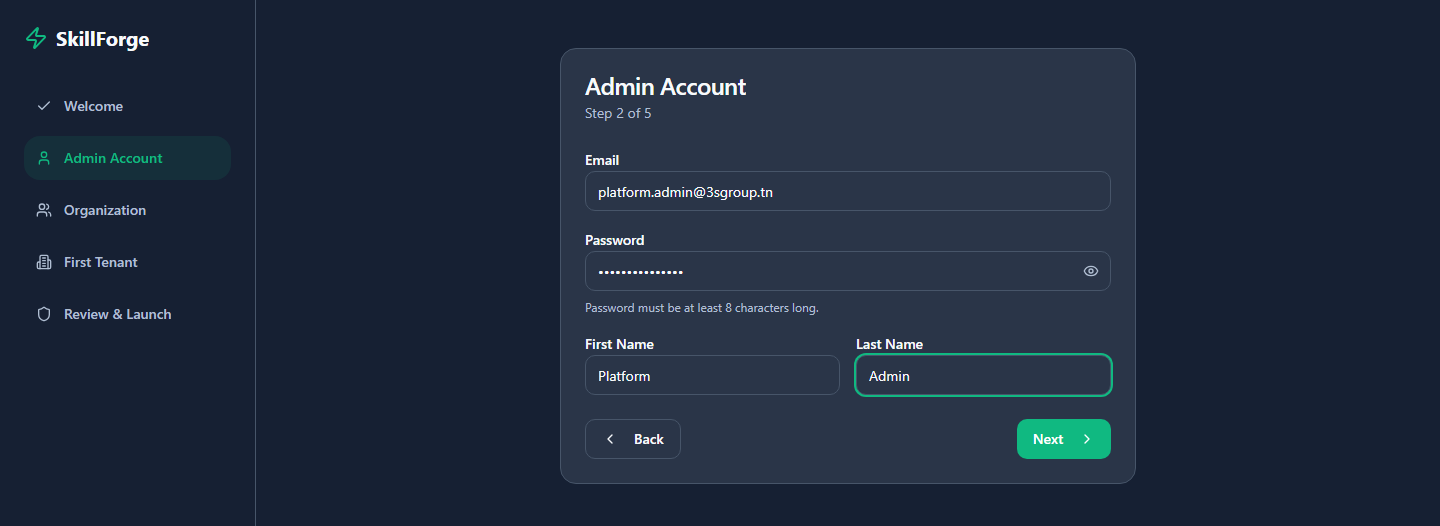
\includegraphics[width=0.92\textwidth]{figures/ch3_setup_superadmin.png}
    \caption{Interface d'initialisation de la plateforme et création du compte SuperAdmin}
    \label{fig:ch3_setup_superadmin}
\end{figure}

\subsubsection{Gestion des tenants et isolation multi-tenant}

La plateforme adopte une architecture multi-tenant permettant à plusieurs entreprises de partager la même infrastructure tout en conservant une séparation logique de leurs données. Chaque entreprise est représentée par un tenant disposant de sa propre configuration.

L'isolation est assurée par l'attribut \texttt{tenant\_id}, associé aux utilisateurs et transmis dans les jetons d'accès. Les services backend utilisent cet identifiant pour restreindre l'accès aux ressources de chaque organisation (utilisateurs, cours, équipes, progression, etc.).

Le SuperAdmin dispose d'une vue globale lui permettant de gérer les différents tenants, notamment leur création, leur activation et leur configuration, comme l'illustre la figure~\ref{fig:ch3_multitenant_tenants}.

\begin{figure}[H]
    \centering
    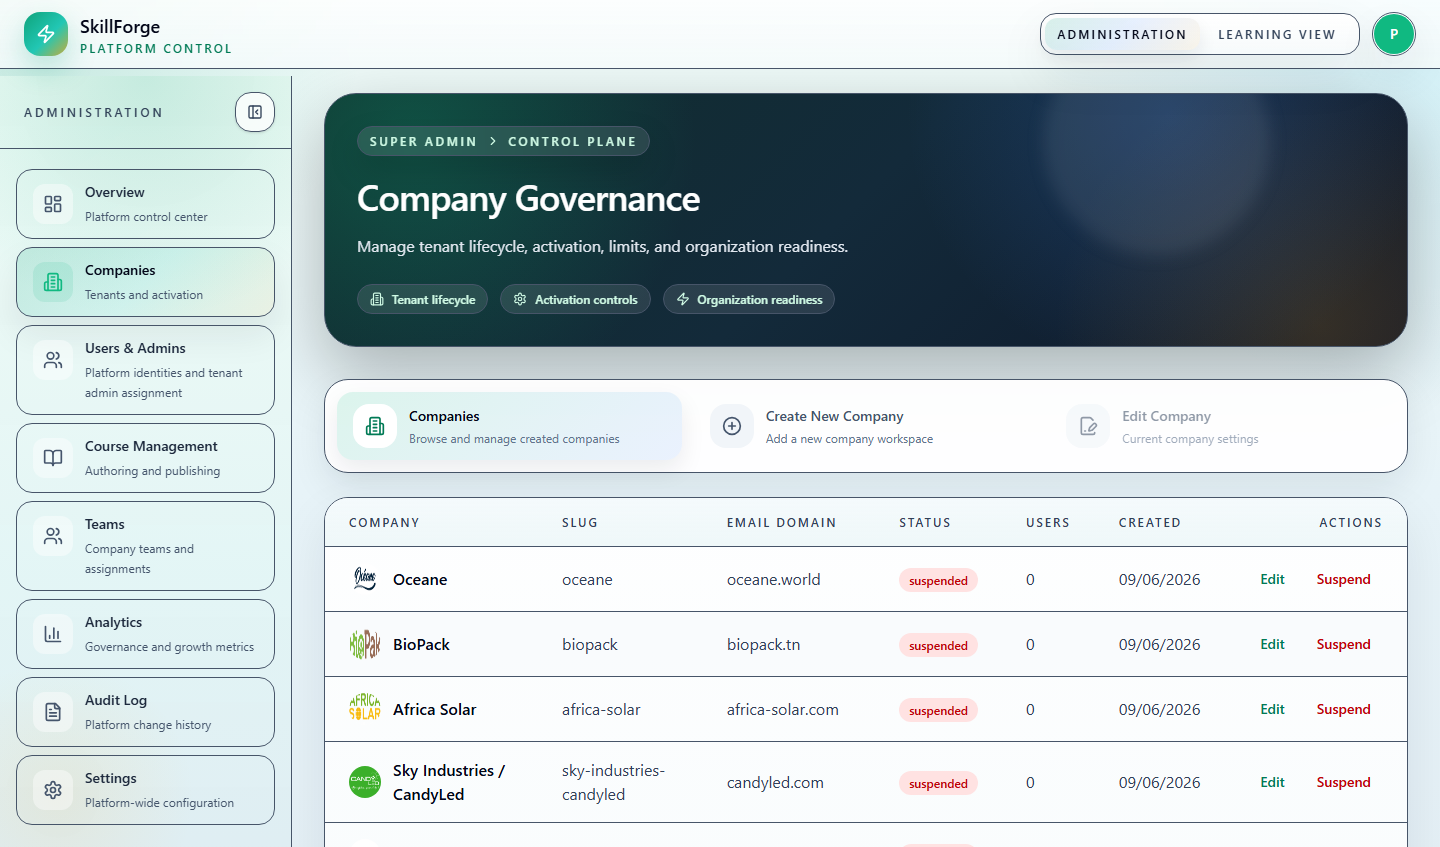
\includegraphics[width=0.92\textwidth]{figures/ch3_multitenant_tenants.png}
    \caption{Gestion multi-tenant des entreprises depuis l'espace SuperAdmin}
    \label{fig:ch3_multitenant_tenants}
\end{figure}

\newpage

La création d'un nouveau tenant se fait à partir d'un formulaire dédié permettant de renseigner les informations principales de l'entreprise, notamment son domaine e-mail, sa limite de sièges et ses paramètres d'identité, comme le montre la figure~\ref{fig:ch3_multitenant_create_tenant}.

\begin{figure}[H]
    \centering
    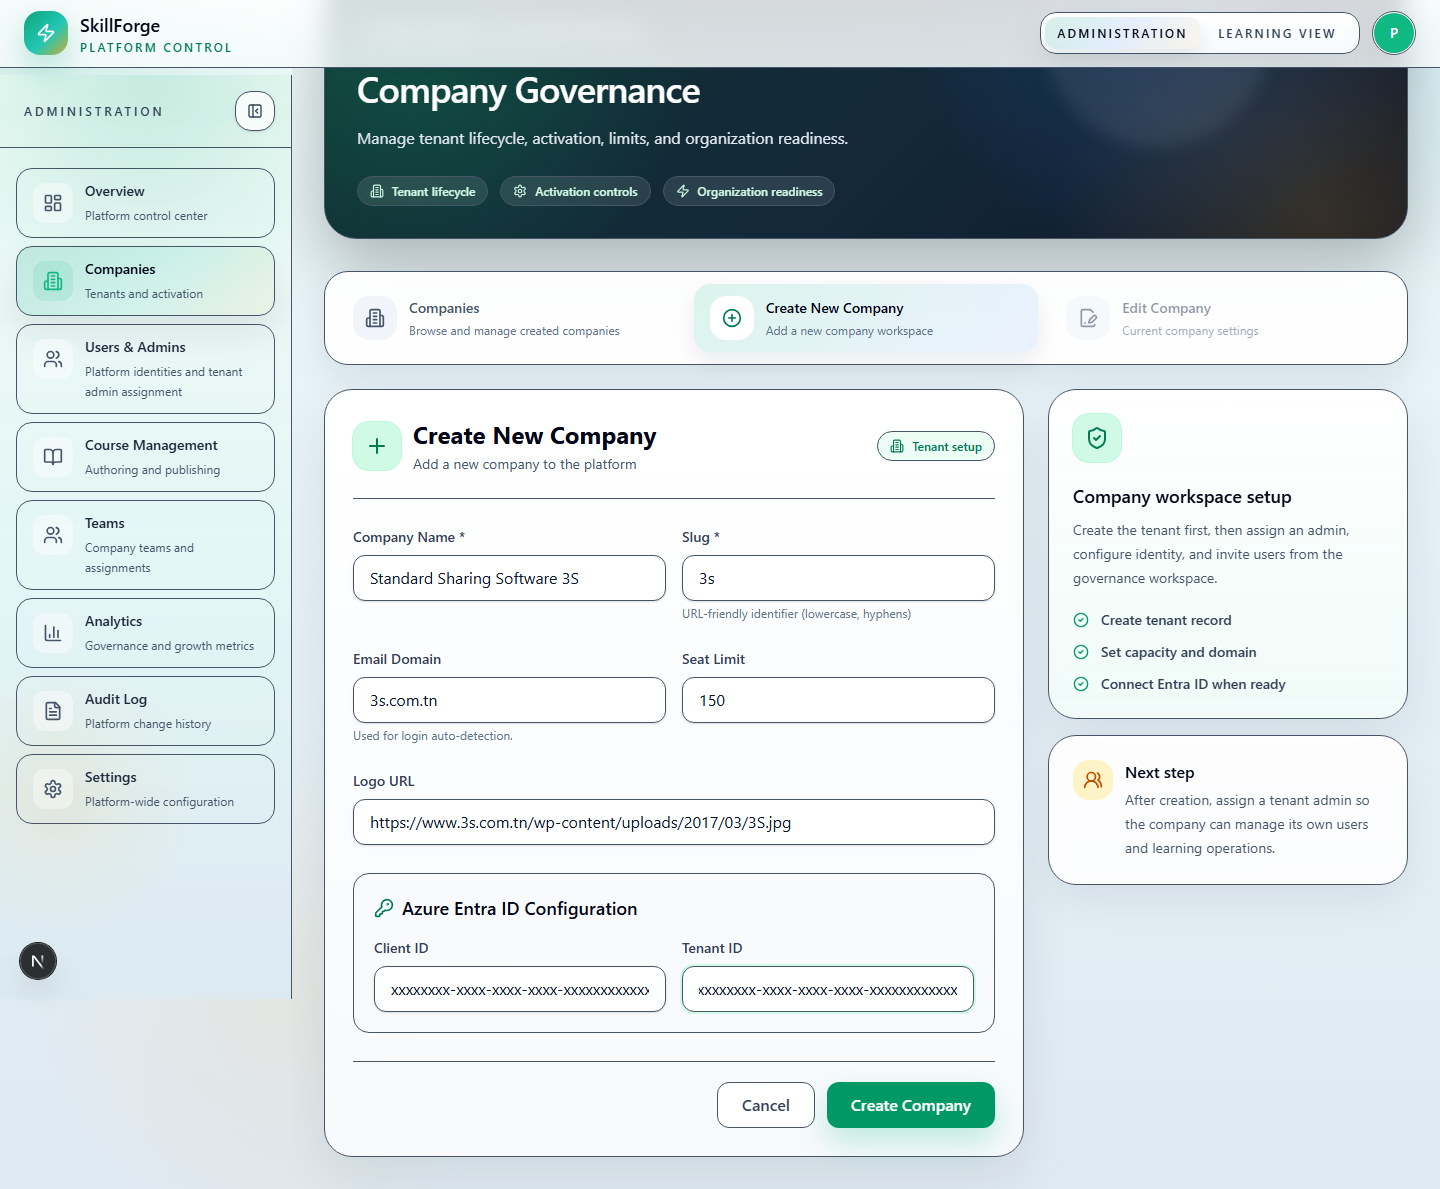
\includegraphics[width=0.92\textwidth]{figures/ch3_multitenant_create_tenant.png}
    \caption{Création d'un tenant avec domaine d'entreprise, limite de sièges et paramètres d'identité}
    \label{fig:ch3_multitenant_create_tenant}
\end{figure}

\subsubsection{Gestion des utilisateurs et des comptes}

Le module \textit{Identity} permet de gérer les comptes utilisateurs rattachés aux tenants. Cette gestion est assurée par le \textit{SuperAdmin} au niveau global de la plateforme et par l'\textit{Admin} au niveau de son entreprise. Ces rôles peuvent créer des comptes, définir le département, attribuer un rôle et suivre le statut des utilisateurs dans leur périmètre d'accès.

La figure~\ref{fig:ch3_identity_users_management} illustre l'interface de gestion des utilisateurs dans l'espace d'administration d'un tenant.

\begin{figure}[H]
    \centering
    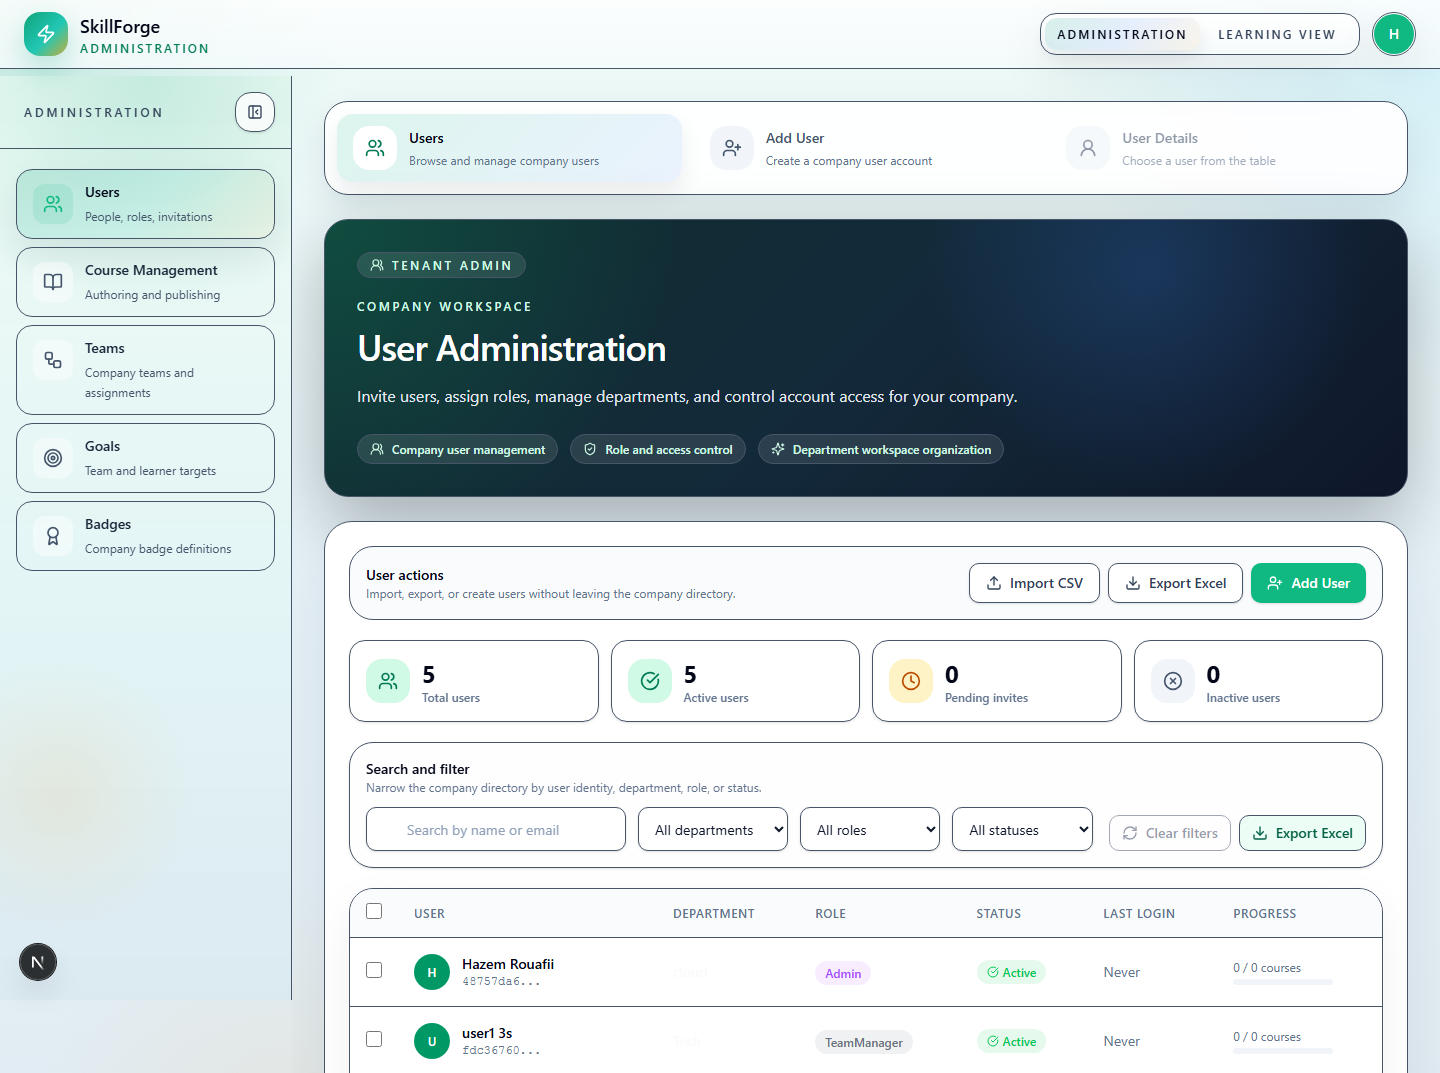
\includegraphics[width=0.92\textwidth]{figures/ch3_identity_users_management.png}
    \caption{Gestion des utilisateurs et des comptes dans l'espace d'administration d'un tenant}
    \label{fig:ch3_identity_users_management}
\end{figure}

\subsubsection{Mécanisme d'authentification}

Le mécanisme d'authentification permet aux utilisateurs rattachés à une entreprise de se connecter à l'aide d'identifiants propres à la plateforme ou, lorsque le tenant est configuré, avec Azure Entra ID via un accès SSO (Single Sign-On, c'est-à-dire une connexion unique avec le compte de l'entreprise). Cette interface de connexion est illustrée par la figure~\ref{fig:ch3_auth_login_tenant}.

Après la connexion, la plateforme détermine le contexte d'accès de l'utilisateur : identité, rôle, statut et tenant associé. Ce contexte permet de rediriger chaque profil vers son espace et d'appliquer les autorisations côté backend à travers des gardes comme \texttt{require\_role}. Les rôles principaux gérés sont SuperAdmin, Admin, LearningExpert, TeamManager et TeamMember.

\begin{figure}[H]
    \centering
    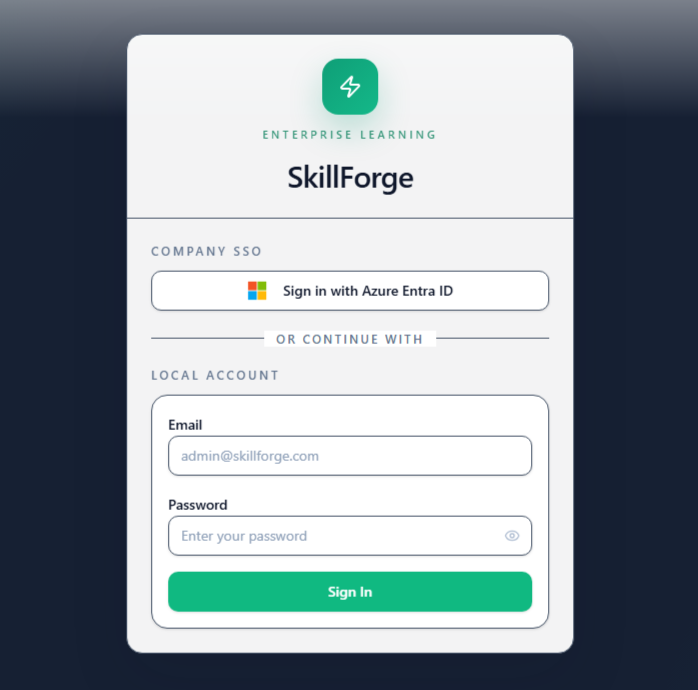
\includegraphics[width=0.50\textwidth]{figures/ch3_auth_login_tenant.png}
    \caption{Interface de connexion avec authentification applicative et option Azure Entra ID}
    \label{fig:ch3_auth_login_tenant}
\end{figure}

\subsubsection{Gestion des sessions et des jetons d'accès}

Lors d'une connexion réussie, le module \textit{Identity} génère un \textit{access token} et un \textit{refresh token}. L'\textit{access token} autorise les appels aux API protégées et transporte le contexte minimal de sécurité, notamment l'utilisateur, son rôle et son tenant.

Le \textit{refresh token} permet de renouveler la session sans demander une nouvelle connexion à chaque expiration de l'\textit{access token}. Cette séparation maintient l'expérience utilisateur tout en limitant la durée de validité du jeton utilisé pour accéder aux ressources sensibles.


\subsubsection{Traçabilité et audit des actions d'administration}

Afin de renforcer la gouvernance de la plateforme, le module Identity conserve des traces des actions sensibles réalisées dans les espaces d'administration. Ces traces permettent de suivre les opérations liées aux tenants, aux comptes utilisateurs, aux changements de statut et aux actions effectuées par les administrateurs.

Cette traçabilité est importante dans un contexte multi-tenant, car elle permet de distinguer les actions globales du SuperAdmin des actions propres à une entreprise. La figure~\ref{fig:ch3_identity_audit_trail} illustre l'interface utilisée pour consulter ces traces.

\begin{figure}[H]
    \centering
    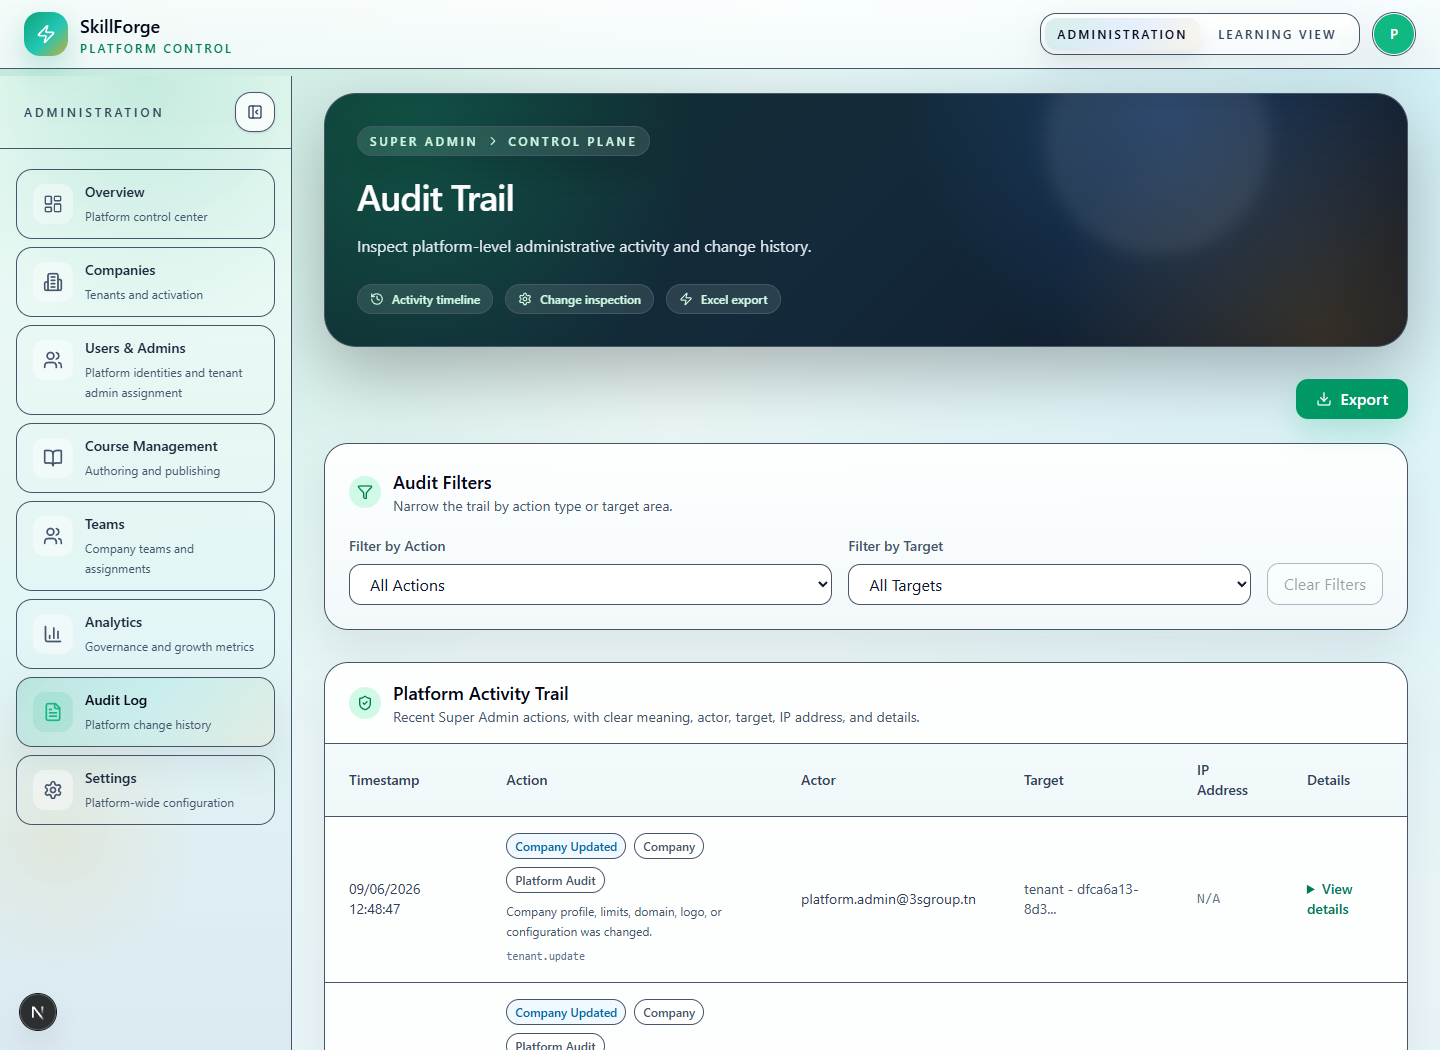
\includegraphics[width=0.92\textwidth]{figures/ch3_identity_audit_trail.png}
    \caption{Consultation des traces d'audit des actions d'administration}
    \label{fig:ch3_identity_audit_trail}
\end{figure}

\subsection{Gestion des formations, cours et progression}

Le module \textit{Learning} regroupe les fonctionnalités liées au parcours pédagogique des utilisateurs. Il couvre la création et l'organisation des cours, l'inscription des apprenants, le suivi de la progression et la mise à jour des objectifs d'apprentissage. Les données produites par ce module alimentent aussi d'autres parties de la plateforme, notamment la gamification, les notifications et les agents IA.

\subsubsection{Gestion administrative et création des cours}

Les utilisateurs autorisés, notamment le \textit{SuperAdmin}, l'\textit{Admin} et le \textit{LearningExpert}, disposent d'interfaces pour créer et gérer les cours. Le \textit{SuperAdmin} peut intervenir à l'échelle globale de la plateforme, tandis que l'\textit{Admin} et le \textit{LearningExpert} agissent dans le périmètre de leur tenant. Cette gestion permet de renseigner les informations principales du cours, de modifier son contenu, de suivre son état et de le publier lorsqu'il est prêt à être consulté par les apprenants.

Deux modes de création sont pris en charge :
\begin{itemize}
    \item \textbf{Mode traditionnel :} le responsable crée manuellement le cours en renseignant ses informations principales, telles que le titre, la description, le niveau, la catégorie ainsi que le nombre de points attribués à l'apprenant après sa complétion, comme l'illustre la figure~\ref{fig:ch3_learning_traditional_course_form}.

Il définit ensuite la structure pédagogique du cours en organisant les leçons, les ressources et les évaluations. Chaque leçon peut contenir du contenu pédagogique, des supports vidéo ainsi que des ressources complémentaires. Le responsable peut également ajouter des quiz afin d'évaluer la compréhension des apprenants et d'assurer un suivi mesurable de leur progression. Cette organisation est illustrée par la figure~\ref{fig:ch3_learning_traditional_course_structure}.

    \begin{figure}[H]
        \centering
        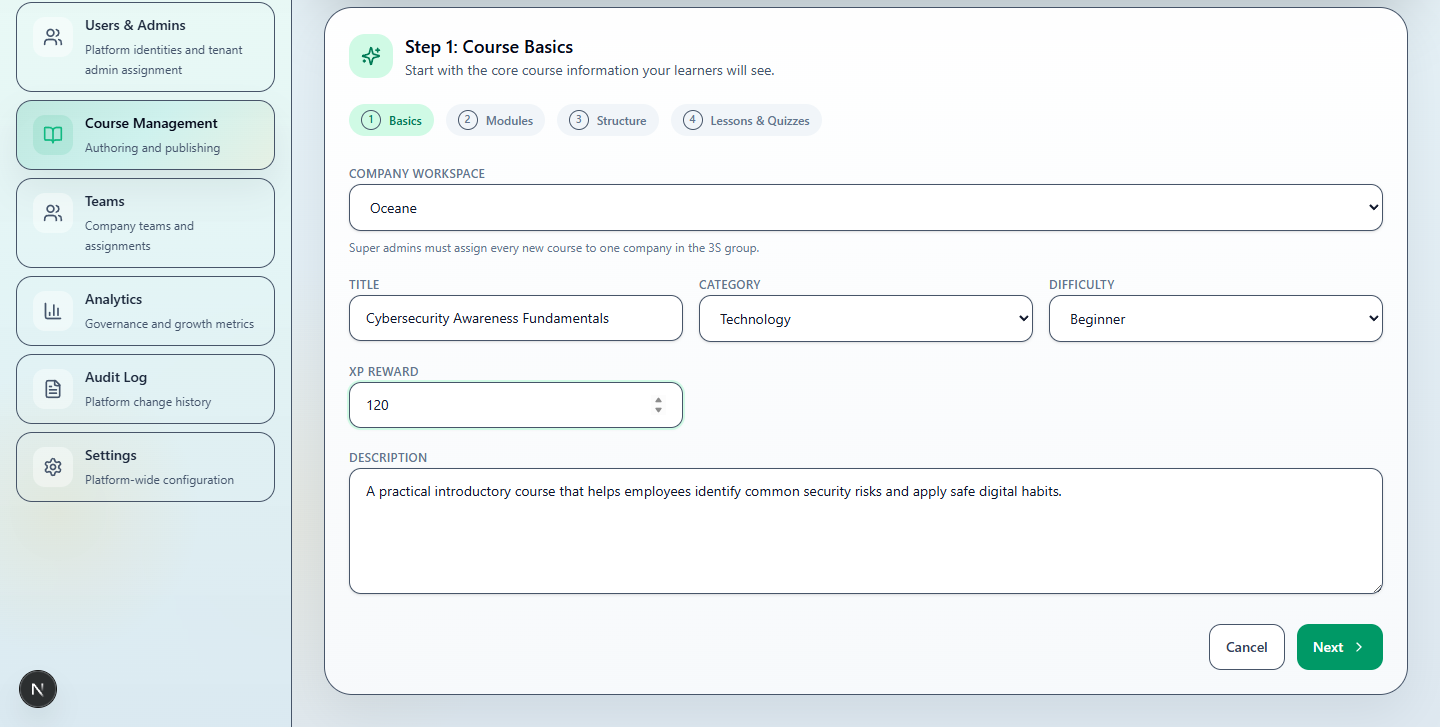
\includegraphics[width=0.9\textwidth]{figures/ch3_learning_traditional_course_form.png}
        \caption{Formulaire de création d'un cours traditionnel dans l'espace d'administration}
        \label{fig:ch3_learning_traditional_course_form}
    \end{figure}

    \begin{figure}[H]
        \centering
        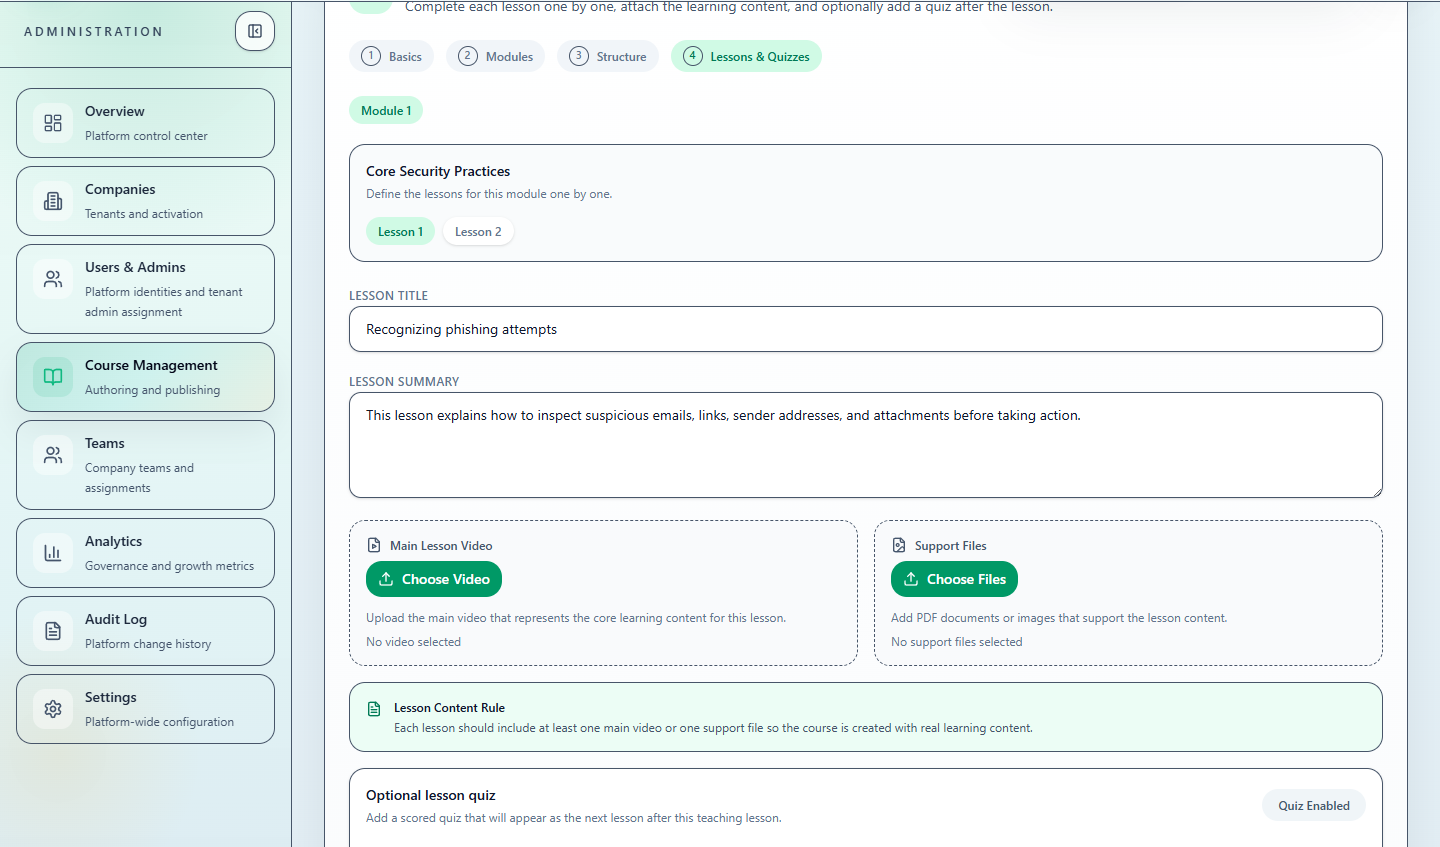
\includegraphics[width=0.92\textwidth]{figures/ch3_learning_traditional_course_structure.png}
        \caption{Organisation d'un cours avec ses leçons, vidéos, ressources et quiz}
        \label{fig:ch3_learning_traditional_course_structure}
    \end{figure}

    \item \textbf{Mode \textit{AI generated} :} le responsable pédagogique démarre la création assistée en décrivant le besoin de formation à couvrir. Il renseigne les informations nécessaires à la génération, notamment le sujet du cours, le public cible, le niveau attendu, les objectifs d'apprentissage, les compétences à développer, la durée souhaitée, le nombre de leçons ainsi que, éventuellement, la langue ou certaines consignes spécifiques. La figure~\ref{fig:ch3_learning_ai_course_input} illustre l'interface utilisée pour saisir ce besoin.

À partir de ces informations, la plateforme génère automatiquement un brouillon structuré du cours comprenant le plan global, les objectifs pédagogiques, les leçons proposées, le contenu initial ainsi que des questions de quiz lorsque cela est pertinent.

Afin de faciliter l'adaptation du contenu, la plateforme intègre un assistant IA de révision permettant au responsable pédagogique de demander des modifications en langage naturel via une interface conversationnelle. Il peut ainsi reformuler une section, approfondir une notion, simplifier un passage, ajouter des exemples ou adapter le contenu à un public spécifique. Les modifications sont appliquées directement au brouillon, ce qui réduit les manipulations manuelles et accélère le processus de création.

Le cours généré reste entièrement éditable et sous le contrôle du responsable pédagogique, qui peut vérifier le contenu, effectuer des ajustements complémentaires et valider la cohérence pédagogique avant publication. La figure~\ref{fig:ch3_learning_ai_course_draft_editor} illustre le résultat généré ainsi que les éléments modifiables du cours produit.

    \begin{figure}[H]
        \centering
        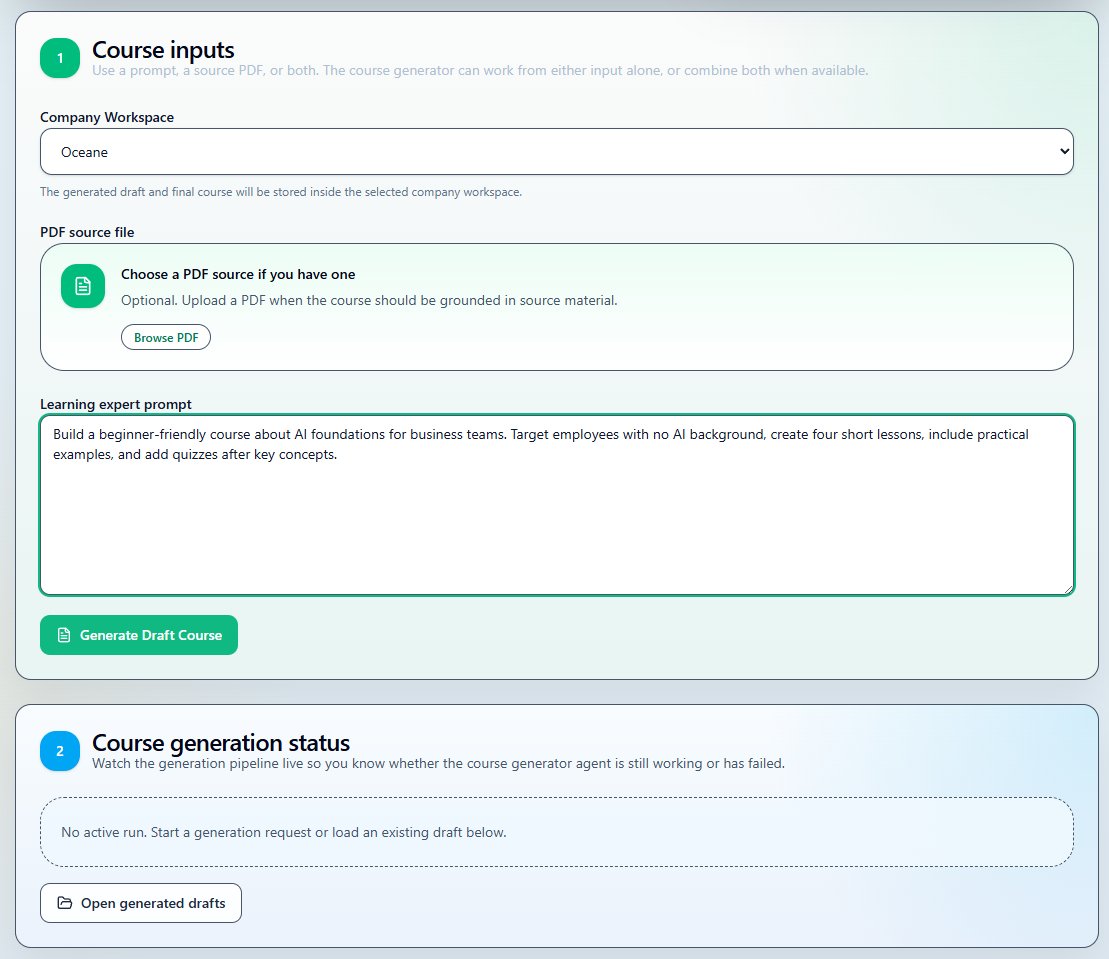
\includegraphics[width=0.72\textwidth]{figures/ch3_learning_ai_course_input.png}
        \caption{Interface de création d'un cours généré par IA avec les champs de saisie du besoin pédagogique}
        \label{fig:ch3_learning_ai_course_input}
    \end{figure}

    \begin{figure}[H]
        \centering
        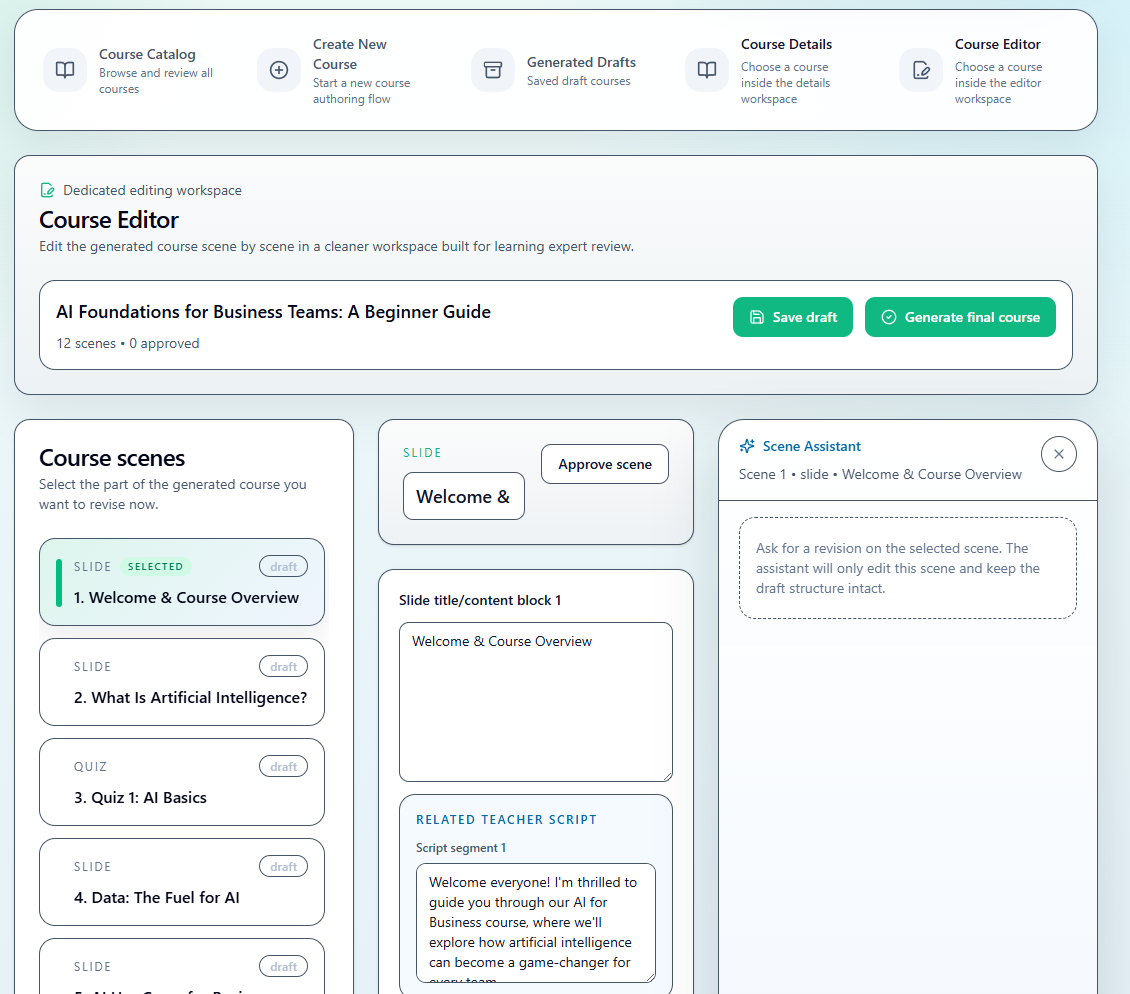
\includegraphics[width=0.82\textwidth]{figures/ch3_learning_ai_course_draft_editor.png}
        \caption{Résultat de génération affichant le brouillon du cours, ses leçons et ses éléments éditables}
        \label{fig:ch3_learning_ai_course_draft_editor}
    \end{figure}
\end{itemize}

\subsubsection{Inscription des apprenants aux cours}

Les apprenants peuvent accéder aux cours publiés dans le périmètre de leur tenant depuis le catalogue de cours, présenté dans la figure~\ref{fig:ch3_learning_course_catalog}. Cette interface permet de consulter les formations disponibles, de filtrer les résultats et d'ouvrir la page détaillée d'un cours.

L'inscription se fait depuis la page de détail du cours, où l'apprenant retrouve les informations principales de la formation, sa durée, son niveau, le nombre de modules et le bouton d'inscription, comme l'illustre la figure~\ref{fig:ch3_learning_course_enrollment_action}. Une fois inscrit, le cours apparaît dans l'espace \textit{My Learning}, qui regroupe les formations en cours et les formations terminées, comme le montre la figure~\ref{fig:ch3_learning_my_learning_enrollments}.

\begin{figure}[H]
    \centering
    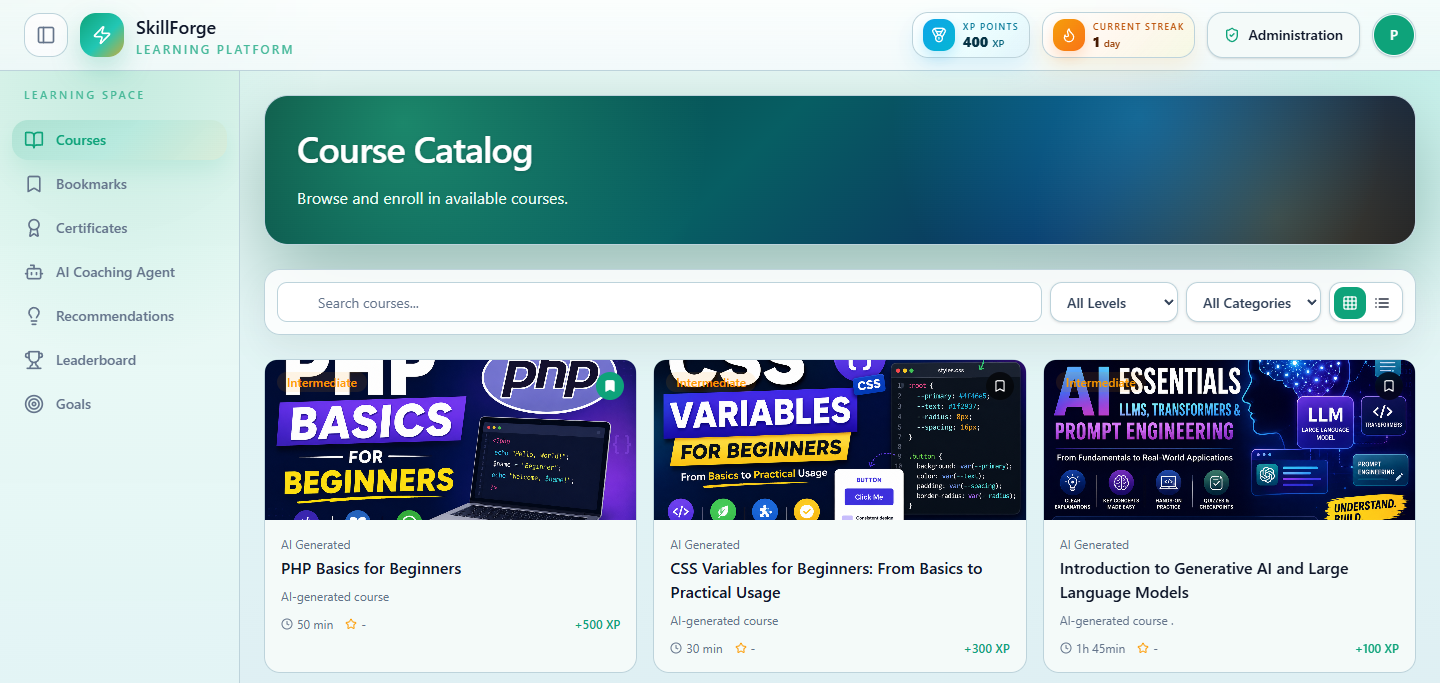
\includegraphics[width=0.82\textwidth]{figures/ch3_learning_course_catalog.png}
    \caption{Catalogue des cours disponibles pour l'apprenant}
    \label{fig:ch3_learning_course_catalog}
\end{figure}

\begin{figure}[H]
    \centering
    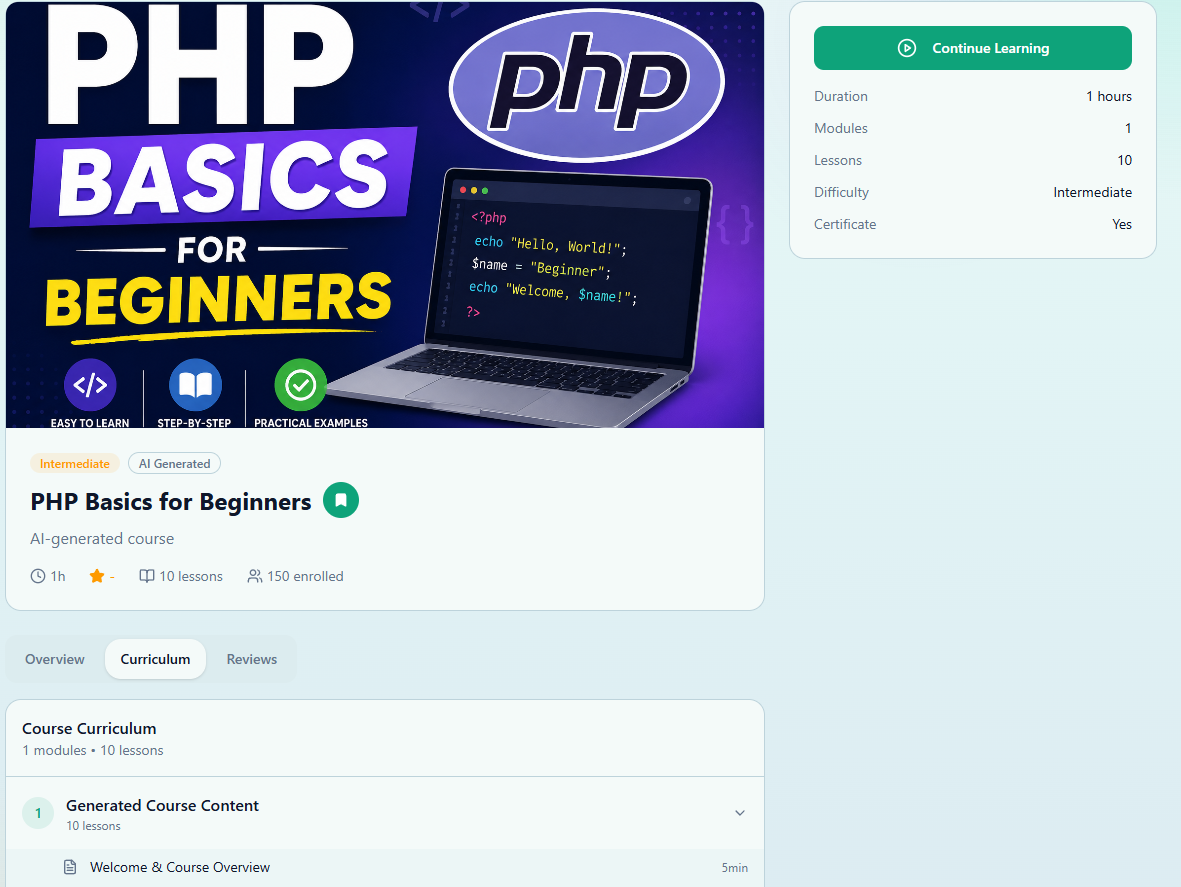
\includegraphics[width=0.62\textwidth]{figures/ch3_learning_course_enrollment_action.png}
    \caption{Page de détail d'un cours avec l'action d'inscription}
    \label{fig:ch3_learning_course_enrollment_action}
\end{figure}

\begin{figure}[H]
    \centering
    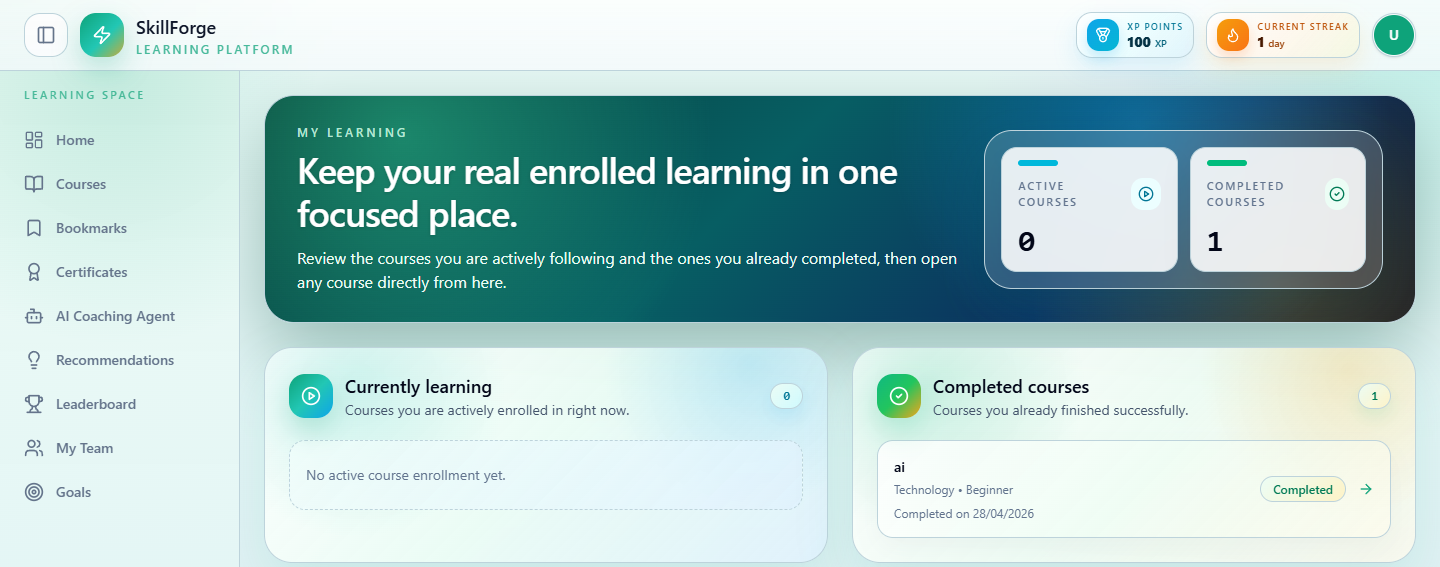
\includegraphics[width=0.82\textwidth]{figures/ch3_learning_my_learning_enrollments.png}
    \caption{Espace My Learning affichant les cours inscrits de l'apprenant}
    \label{fig:ch3_learning_my_learning_enrollments}
\end{figure}

\subsubsection{Suivi de la progression individuelle}

Le suivi de progression repose sur les activités réalisées par l'apprenant, comme la consultation des leçons, leur complétion et l'avancement global dans un cours. Ces informations sont affichées dans la page de progression individuelle, qui regroupe les indicateurs principaux : points d'expérience (XP), niveau, série d'apprentissage, leçons terminées, cours complétés et activités récentes, comme le montre la figure~\ref{fig:ch3_learning_progress_dashboard}.

La progression est aussi visible depuis l'espace \textit{My Learning}, comme illustré en figure~\ref{fig:ch3_learning_my_learning_enrollments}. Cette page distingue les cours en cours des cours terminés, ce qui permet à l'apprenant de reprendre rapidement son parcours ou de consulter les formations déjà finalisées.

Au niveau d'une leçon, la plateforme affiche l'état d'avancement du cours, le nombre de leçons complétées et le statut de chaque leçon. La figure~\ref{fig:ch3_learning_lesson_progress_tracking} illustre ce suivi détaillé dans l'interface de lecture.

\begin{figure}[H]
    \centering
    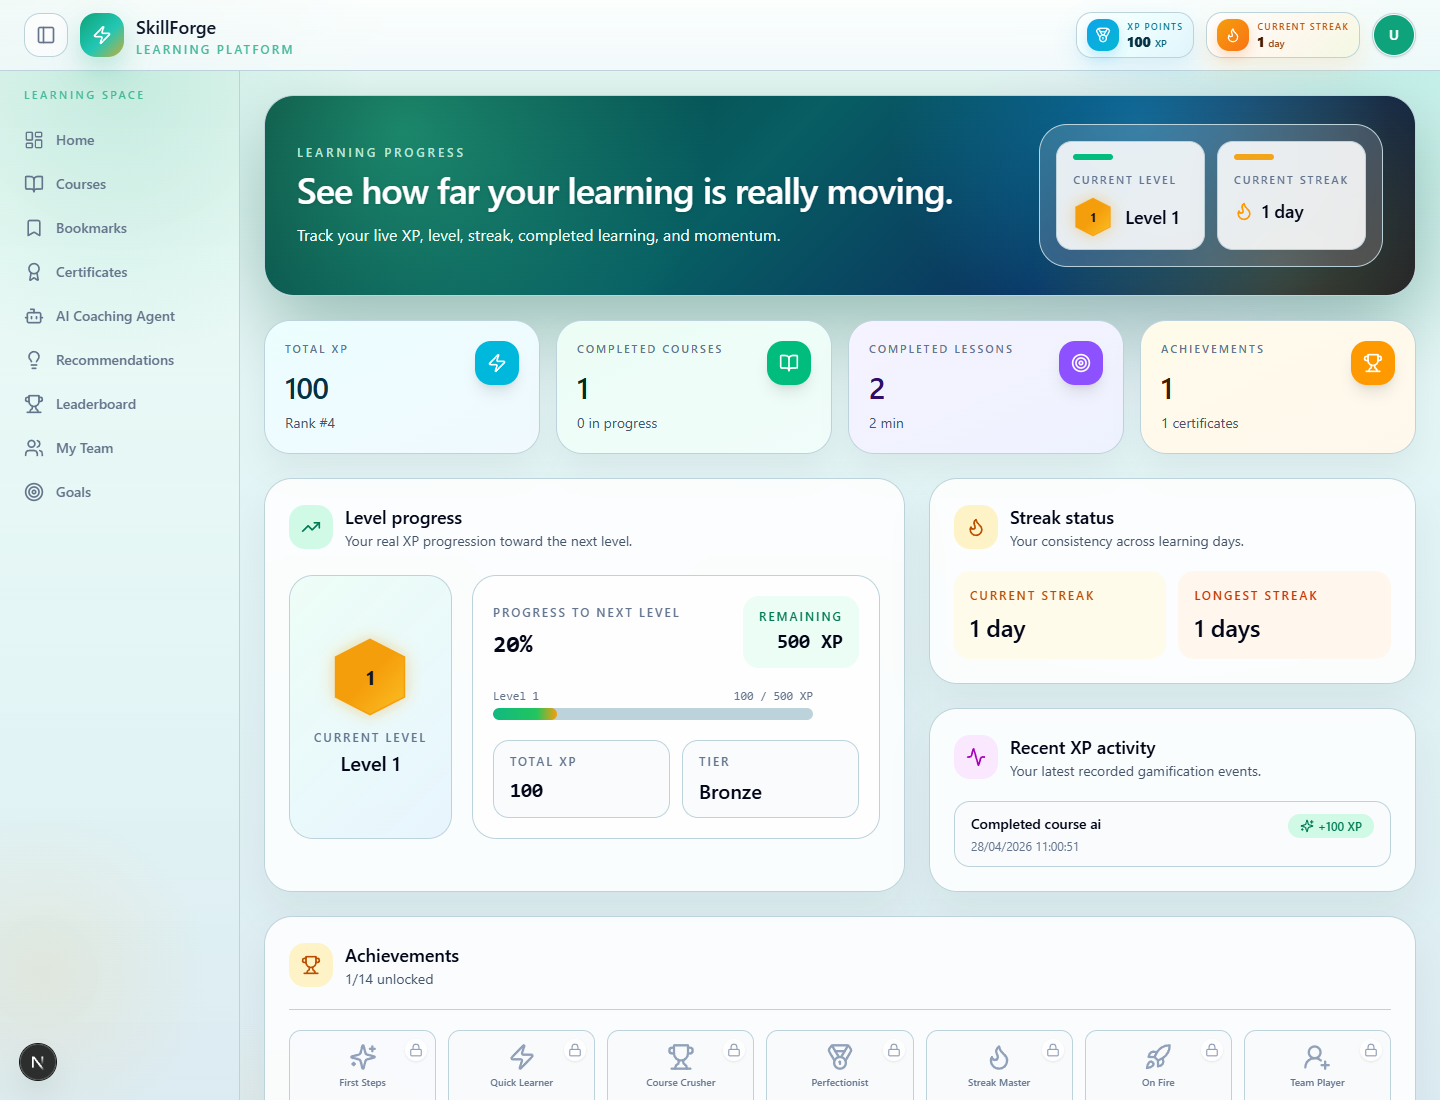
\includegraphics[width=0.82\textwidth]{figures/ch3_learning_progress_dashboard.png}
    \caption{Tableau de progression individuelle affichant les indicateurs d'apprentissage de l'utilisateur}
    \label{fig:ch3_learning_progress_dashboard}
\end{figure}

\begin{figure}[H]
    \centering
    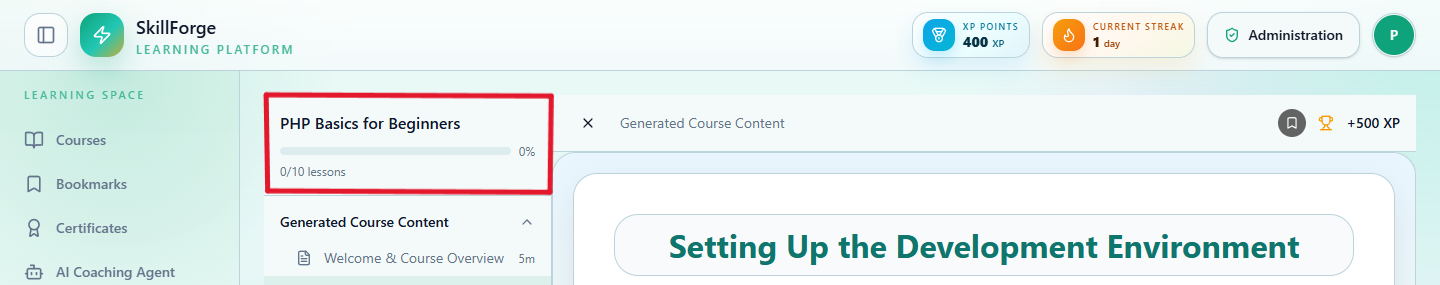
\includegraphics[width=0.82\textwidth]{figures/ch3_learning_lesson_progress_tracking.png}
    \caption{Suivi détaillé de la progression dans une leçon}
    \label{fig:ch3_learning_lesson_progress_tracking}
\end{figure}

\subsubsection{Objectifs d'apprentissage personnels et collectifs}

La plateforme permet aussi de gérer des objectifs d'apprentissage personnels et collectifs. Les objectifs personnels ciblent un utilisateur précis, tandis que les objectifs d'équipe concernent plusieurs membres d'une même équipe. Leur progression peut être mise à jour automatiquement à partir des activités réelles, par exemple le nombre de leçons terminées ou le temps d'étude réalisé, comme le montre la figure~\ref{fig:ch3_learning_goals_tracking}.

\begin{figure}[H]
    \centering
    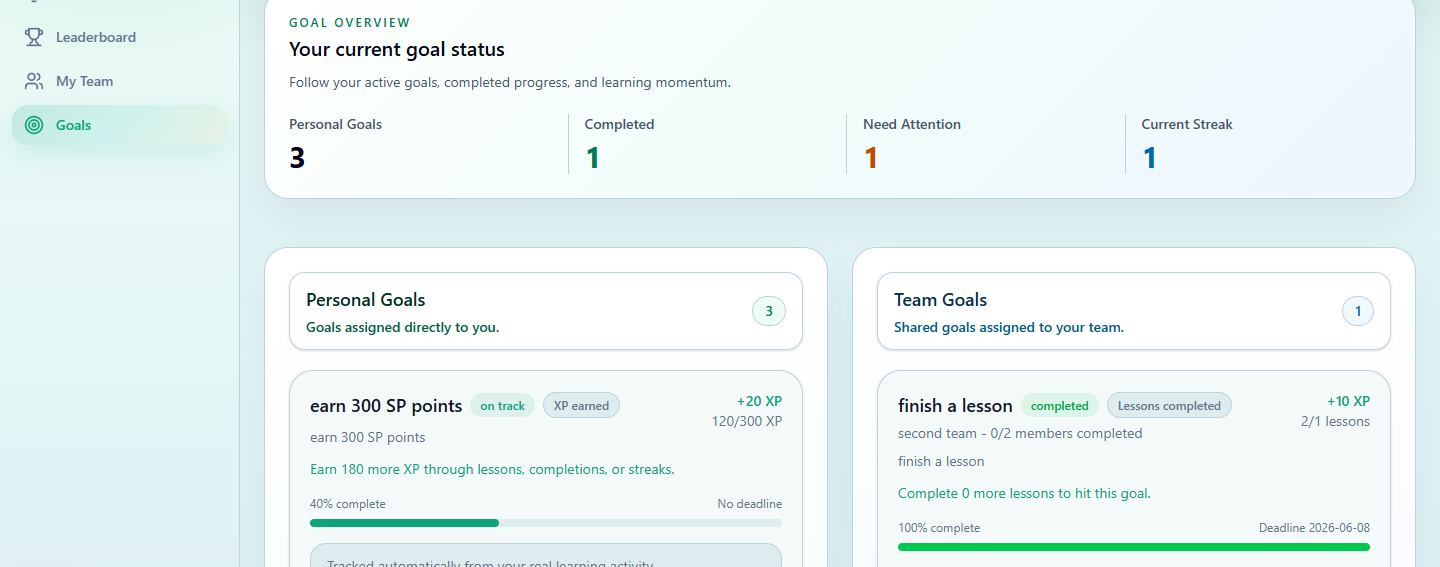
\includegraphics[width=0.92\textwidth]{figures/ch3_learning_goals_tracking.png}
    \caption{Interface de suivi des objectifs personnels et des objectifs d'équipe}
    \label{fig:ch3_learning_goals_tracking}
\end{figure}

\subsubsection{Certificats de fin de cours et vérification}

À la fin d'un cours, la plateforme délivre un certificat à l'apprenant lorsque les conditions de complétion sont satisfaites, à savoir la validation de l'ensemble des leçons et la réussite des quiz associés avec un score minimum de 90~\%. Ce certificat constitue une preuve officielle de réussite et de validation du parcours suivi. Il est accessible depuis l'espace personnel de l'utilisateur et contient les informations essentielles liées à l'apprenant, au cours et à la date d'obtention.

La plateforme propose également un espace dédié à la consultation des certificats, permettant de visualiser l'ensemble des certificats obtenus après la complétion des cours (voir figure~\ref{fig:certificate_list}). Chaque certificat peut être consulté en détail (voir figure~\ref{fig:certificate_detail}), et une interface de vérification permet d'en contrôler l'authenticité à partir de son identifiant ou de son lien de vérification.

\begin{figure}[H]
    \centering
    
\includegraphics[width=0.75\textwidth]{figures/espace_certificate.png}
    \caption{Liste des certificats obtenus par l'apprenant}
    \label{fig:certificate_list}
\end{figure}

\begin{figure}[H]
    \centering
    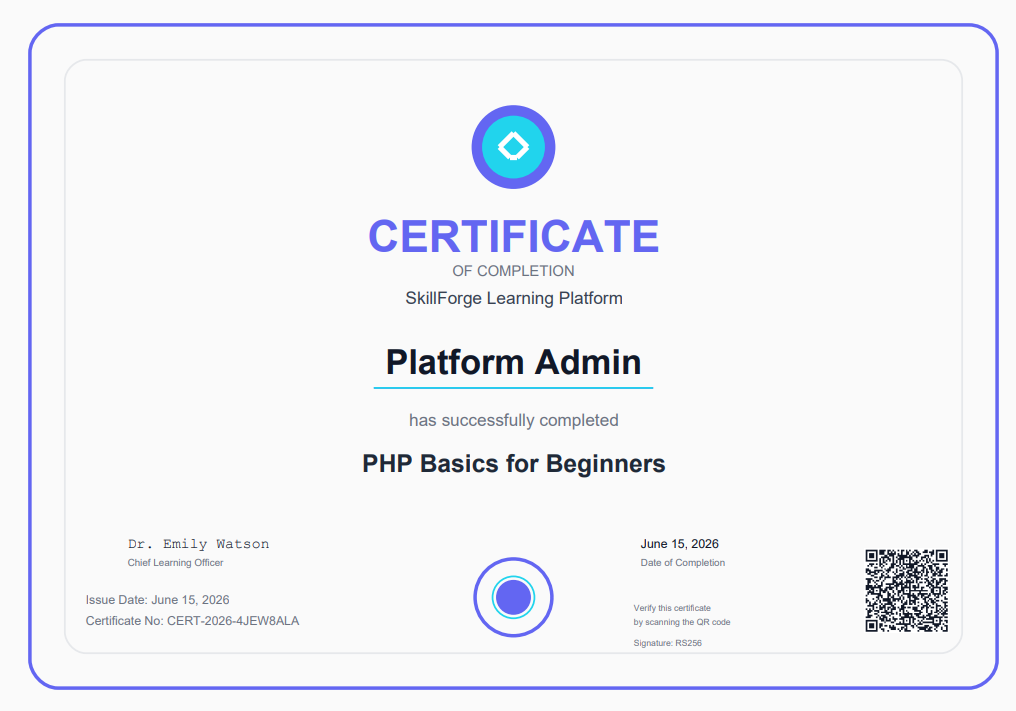
\includegraphics[width=0.72\textwidth]{figures/certificate.png}
    \caption{Détail d'un certificat délivré}
    \label{fig:certificate_detail}
\end{figure}

\paragraph{Mécanisme de sécurité et de vérification}

Afin de garantir l'intégrité des certificats, la plateforme repose sur une signature numérique basée sur l'algorithme \textbf{RS256} (RSA avec SHA-256) :

\begin{itemize}
    \item \textbf{Hachage SHA-256 :} les données du certificat sont sérialisées et hashées pour produire un \textit{content\_hash}.
    \item \textbf{Signature RS256 :} le contenu du certificat est signé avec une clé privée RSA, et la signature est stockée en base.
    \item \textbf{Vérification :} lors de la consultation, le système recalcule le hash, vérifie la signature via la clé publique et contrôle l'état du certificat (validité, révocation).
    \item \textbf{QR code :} chaque certificat est associé à un QR code pointant vers une URL de vérification (\texttt{/verify/\{id\}}), permettant un contrôle rapide de son authenticité. La figure~\ref{fig:certificate_verify} illustre le processus de vérification après scan du QR code ainsi que l'affichage du résultat de validation du certificat.
\end{itemize}

Ainsi, toute modification des données invalide automatiquement la signature, empêchant toute falsification. La clé privée est sécurisée via une variable d'environnement (\texttt{CERT\_PRIVATE\_KEY}).

\begin{figure}[H]
    \centering
    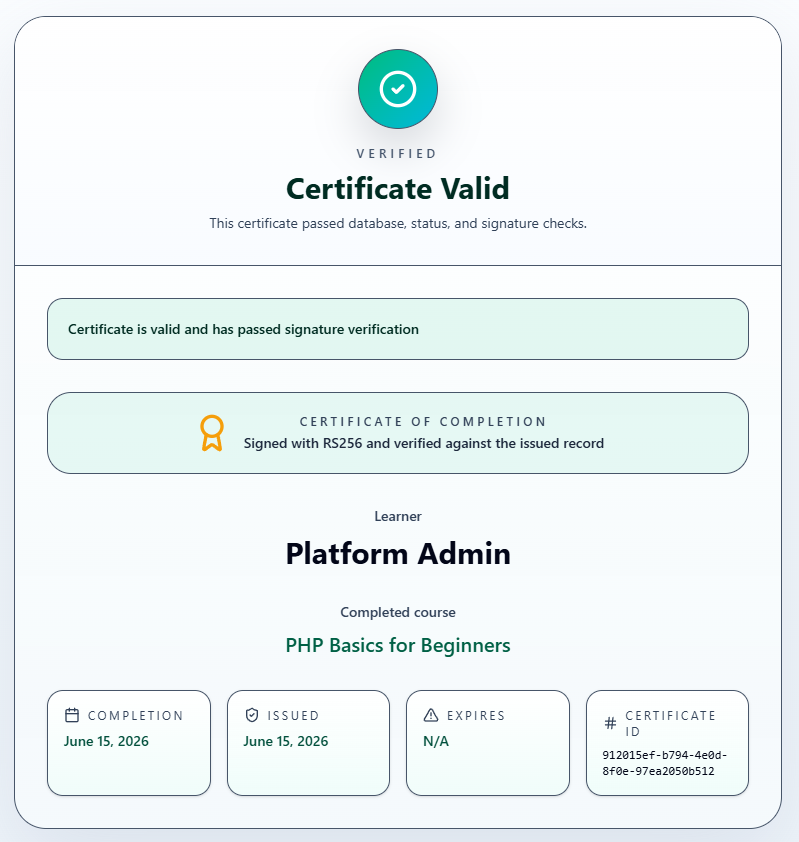
\includegraphics[width=0.58\textwidth]{figures/validation_certificat.png}
    \caption{Page de vérification publique d'un certificat après scan du QR code}
    \label{fig:certificate_verify}
\end{figure}

\subsection{Mentorat et gamification}

Le module de mentorat et de gamification complète le module \textit{Learning} en transformant les activités d'apprentissage en indicateurs de suivi et en éléments de motivation. Il permet de suivre la progression des apprenants, de valoriser leurs réussites et d'encourager leur engagement à travers les points XP, les niveaux, les badges, les objectifs et les classements.

\begin{itemize}
    \item \textbf{Suivi de la progression et du niveau de l'apprenant}

    La plateforme affiche un tableau de progression permettant à l'utilisateur de suivre son niveau actuel, ses points XP (figure~\ref{fig:xp_obtention}), sa série d'apprentissage ainsi que l’état d’avancement vers le niveau suivant. Le tableau de progression présenté en figure~\ref{fig:ch3_learning_progress_dashboard}, constitue également la base du système de gamification, car les indicateurs affichés sont utilisés pour calculer les niveaux, les récompenses et la progression globale de l’apprenant.

    \begin{figure}[H]
        \centering
        \IfFileExists{figures/xp.png}{%
            
\includegraphics[width=0.58\textwidth]{figures/xp.png}%
        }{%
            \fbox{\parbox{0.85\textwidth}{\centering Capture à ajouter : illustration de l'obtention des points XP.}}%
        }
        \caption{Illustration de l'obtention des points XP}
        \label{fig:xp_obtention}
    \end{figure}

    \item \textbf{Badges et reconnaissance des réussites}

    Les badges matérialisent les réussites obtenues par les utilisateurs. Ils peuvent être liés à la complétion d'un cours, à l'atteinte d'un objectif, à une performance particulière ou à la participation à un challenge. L'apprenant peut consulter les badges obtenus et ceux qui restent à débloquer depuis son espace de progression, comme l'illustre la figure~\ref{fig:ch3_gamification_badges}.

    \begin{figure}[H]
        \centering
        \IfFileExists{figures/ch3_gamification_badges.png}{%
            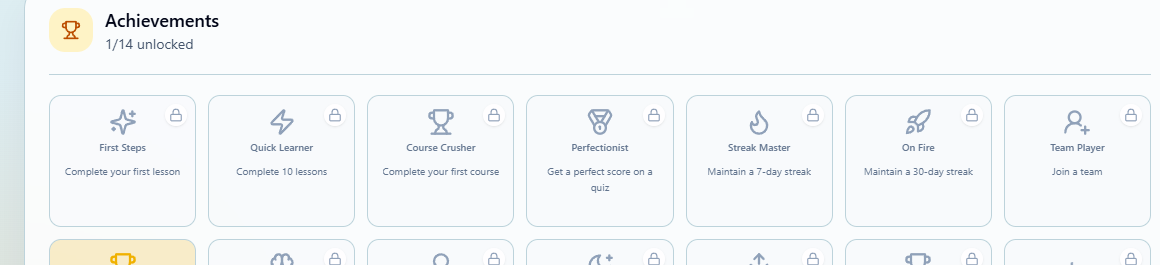
\includegraphics[width=0.92\textwidth]{figures/ch3_gamification_badges.png}%
        }{%
            \fbox{\parbox{0.85\textwidth}{\centering Capture à ajouter : badges obtenus et non encore débloqués.}}%
        }
        \caption{Affichage des badges obtenus et non encore débloqués}
        \label{fig:ch3_gamification_badges}
    \end{figure}

    \item \textbf{Création et gestion des badges personnalisés}

    Les badges personnalisés peuvent être créés par les rôles autorisés, notamment l'administrateur, le \textit{Learning Expert} et le \textit{Team Manager}. Chaque badge est rattaché au tenant de l'entreprise, ce qui garantit que les badges créés dans une société ne sont pas visibles par les autres sociétés. L'interface de gestion des badges permet de définir le nom, le niveau, la condition d'obtention et le contexte d'utilisation du badge, comme le montre la figure~\ref{fig:ch3_gamification_badge_management}.

    \begin{figure}[H]
        \centering
        \IfFileExists{figures/ch3_gamification_badge_management.png}{%
            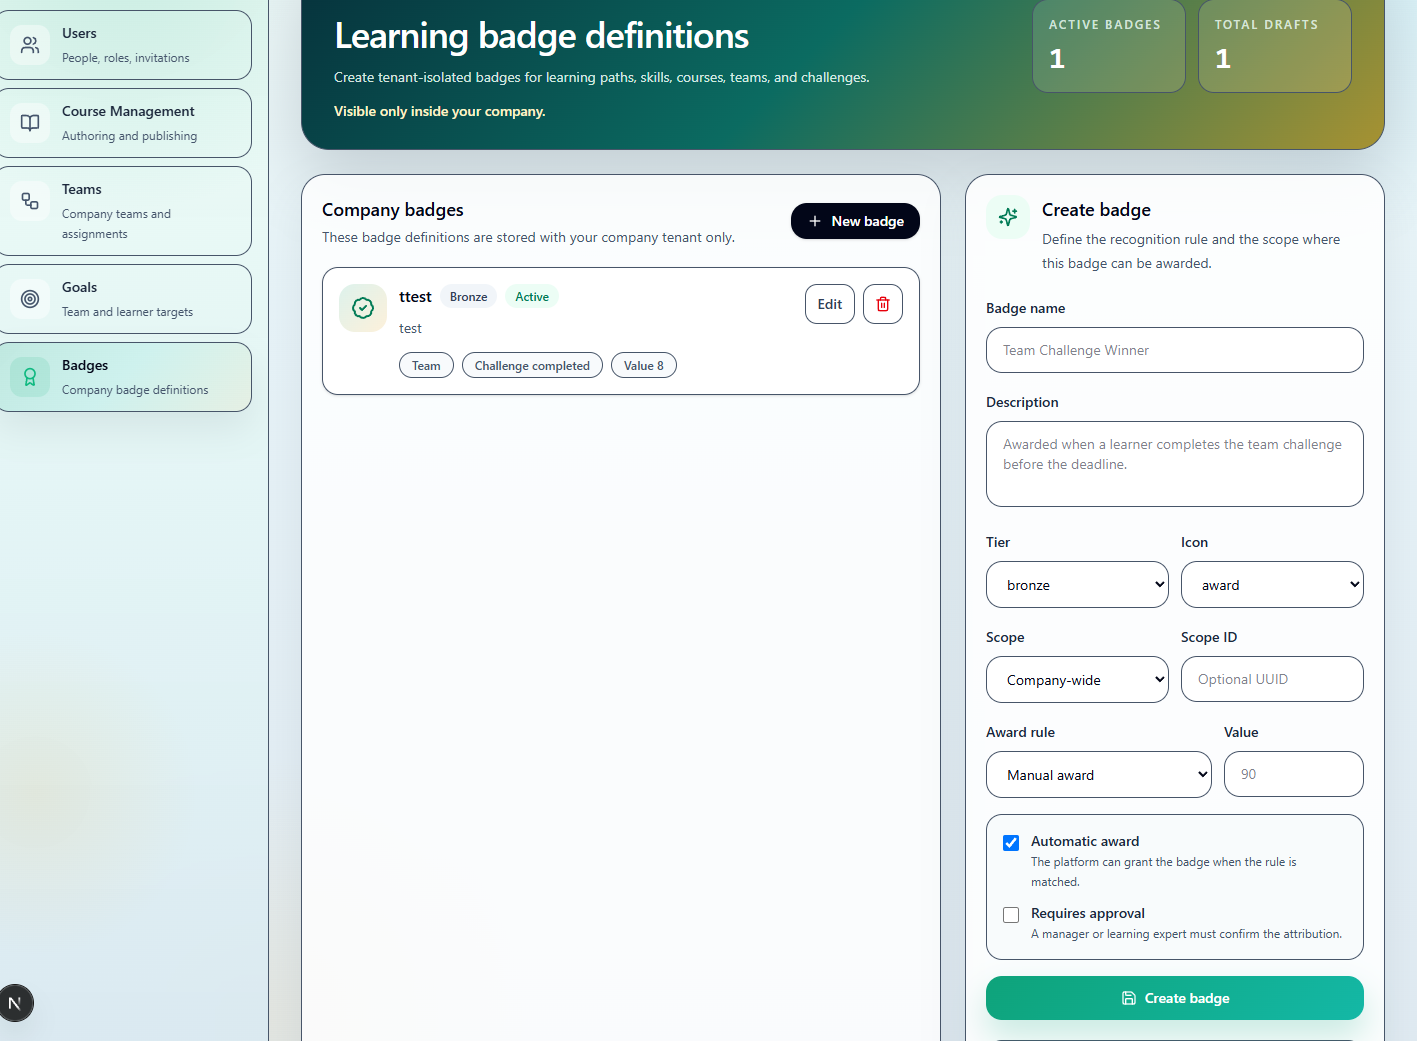
\includegraphics[width=0.8\textwidth]{figures/ch3_gamification_badge_management.png}%
        }{%
            \fbox{\parbox{0.85\textwidth}{\centering Capture à ajouter : interface de gestion des badges personnalisés.}}%
        }
        \caption{Interface de gestion des badges personnalisés}
        \label{fig:ch3_gamification_badge_management}
    \end{figure}

    \item \textbf{Classement des apprenants}

    Le classement permet de comparer la progression des utilisateurs selon leurs points XP, leur niveau et leur activité d'apprentissage. Il offre une vue synthétique de la dynamique d'engagement au sein de la plateforme et peut être utilisé pour suivre la progression globale des apprenants ou des équipes, comme le présente la figure~\ref{fig:ch3_gamification_leaderboard}.

    \begin{figure}[H]
        \centering
        \IfFileExists{figures/ch3_gamification_leaderboard.png}{%
            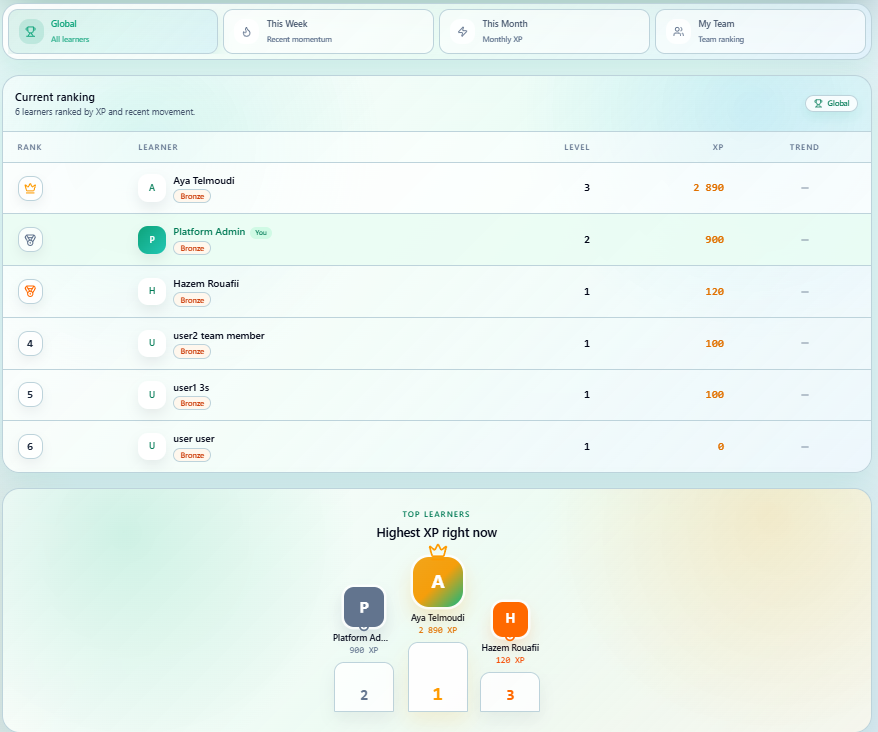
\includegraphics[width=0.92\textwidth]{figures/ch3_gamification_leaderboard.png}%
        }{%
            \fbox{\parbox{0.85\textwidth}{\centering Capture à ajouter : classement des apprenants selon leur progression.}}%
        }
        \caption{Classement des apprenants selon leur progression}
        \label{fig:ch3_gamification_leaderboard}
    \end{figure}
\end{itemize}

\subsection{Modules IA -- les 5 agents}

Les modules IA constituent la partie intelligente de la plateforme. Ils interviennent à différents moments du parcours : création de cours, mémorisation des signaux d'apprentissage, accompagnement personnalisé, recommandation de contenus et génération de challenges. Ces agents sont intégrés à l'application à travers des routes API dédiées et des services AgentOS séparés. Ils s'appuient sur les données du module \textit{Learning}, sur le contexte du tenant et sur le système de mémoire persistante afin de produire des réponses adaptées au profil de l'utilisateur.

\begin{itemize}
    \item \textbf{Agent de génération de cours}

    L'agent de génération de cours assiste les responsables pédagogiques dans la création d'un brouillon de cours à partir d'un besoin exprimé. Il reçoit les informations saisies dans l'interface, comme le sujet, le public cible, le niveau, les objectifs et les contraintes pédagogiques, puis transmet ces éléments au workflow de génération. Le résultat produit est un brouillon structuré composé d'un plan, de leçons et d'éléments éditables. Ce contenu n'est pas publié automatiquement : il doit être relu, corrigé et validé par un utilisateur autorisé avant son intégration dans le catalogue.

    Le résultat éditable produit par cet agent a déjà été présenté dans la figure~\ref{fig:ch3_learning_ai_course_draft_editor}, qui montre le brouillon généré, ses leçons et ses éléments modifiables.

    \item \textbf{Agent de mémoire apprenant}

    L'agent de mémoire apprenant conserve les informations utiles issues des activités réelles de l'utilisateur. Il peut exploiter des événements tels que la complétion d'une leçon, le résultat d'un quiz, une difficulté exprimée dans une discussion ou une réponse donnée lors d'un challenge. Ces informations sont transformées en traces durables et rattachées au bon contexte : utilisateur, tenant, cours et leçon. Cette mémoire permet ensuite aux autres agents de personnaliser leurs réponses au lieu de se limiter à une interaction isolée.

    \item \textbf{Agent de coaching IA}

    L'agent de coaching IA accompagne l'apprenant pendant son parcours. Il peut être utilisé depuis la page de leçon ou depuis l'espace dédié au coaching. Lorsqu'un utilisateur pose une question, l'agent reçoit le contexte du tenant, du cours, de la leçon et de la session de discussion. Il interroge ensuite la mémoire disponible afin de produire une réponse contextualisée, liée au contenu du cours et aux difficultés déjà observées chez l'apprenant (figure~\ref{fig:ch3_ai_coaching_agent}).

    \begin{figure}[H]
        \centering
        \IfFileExists{figures/ch3_ai_coaching_agent.png}{%
            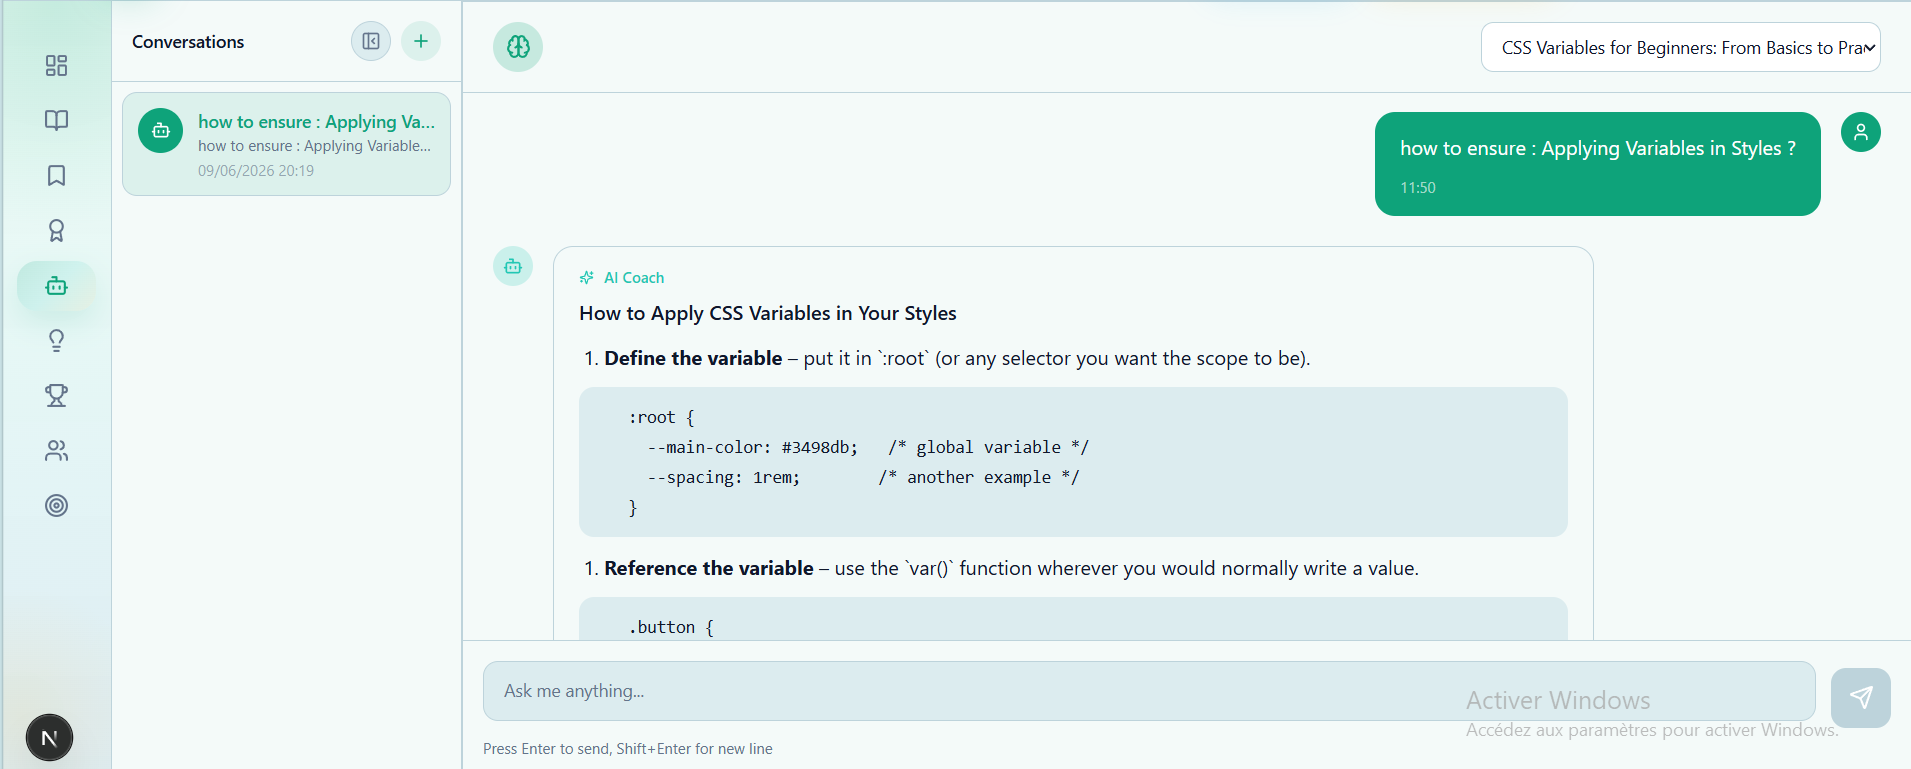
\includegraphics[width=0.95\textwidth]{figures/ch3_ai_coaching_agent.png}%
        }{%
            \fbox{\parbox{0.85\textwidth}{\centering Figure à ajouter : discussion avec l'agent de coaching IA pendant le déroulement d'un cours.}}%
        }
        \caption{Interaction entre l'apprenant et l'agent de coaching IA}
        \label{fig:ch3_ai_coaching_agent}
    \end{figure}

    \item \textbf{Agent de recommandation}

    L'agent de recommandation analyse le profil d'apprentissage de l'utilisateur, ses inscriptions, sa progression, les cours disponibles et les signaux de mémoire pour proposer les prochaines actions pertinentes. Il peut produire des recommandations de cours ou de leçons, mais aussi contribuer à l'identification des écarts de compétences. Son objectif est d'orienter l'apprenant vers les contenus les plus utiles selon son historique et ses objectifs.

    La figure~\ref{fig:ch3_ai_recommendation_agent} devra présenter l'interface des recommandations personnalisées générées pour un apprenant.

    \begin{figure}[H]
        \centering
        \IfFileExists{figures/ch3_ai_recommendation_agent.png}{%
            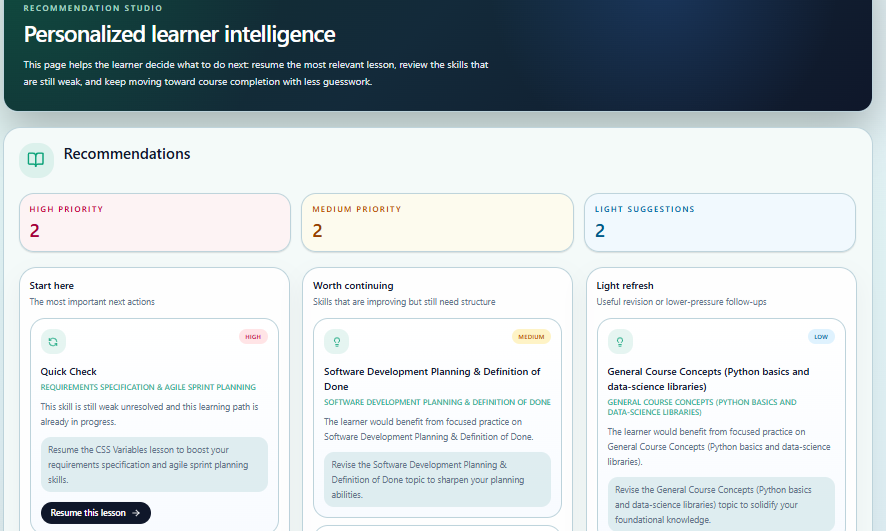
\includegraphics[width=0.92\textwidth]{figures/ch3_ai_recommendation_agent.png}%
        }{%
            \fbox{\parbox{0.85\textwidth}{\centering Figure à ajouter : recommandations personnalisées générées pour un apprenant.}}%
        }
        \caption{Recommandations personnalisées proposées par l'agent IA}
        \label{fig:ch3_ai_recommendation_agent}
    \end{figure}

    \item \textbf{Agent de challenge personnalisé}

    L'agent de challenge personnalisé génère une question ou une activité courte adaptée au contexte d'apprentissage de l'utilisateur. Il peut s'appuyer sur les erreurs de quiz, les difficultés mémorisées ou le cours suivi récemment afin de proposer un exercice ciblé. Après la réponse de l'apprenant, le résultat peut être utilisé pour mettre à jour la progression, attribuer des récompenses et enrichir la mémoire apprenant.

    La figure~\ref{fig:ch3_ai_solo_challenge_agent} devra illustrer l'affichage d'un challenge personnalisé et son retour après réponse.

    \begin{figure}[H]
        \centering
        \IfFileExists{figures/ch3_ai_solo_challenge_agent.png}{%
            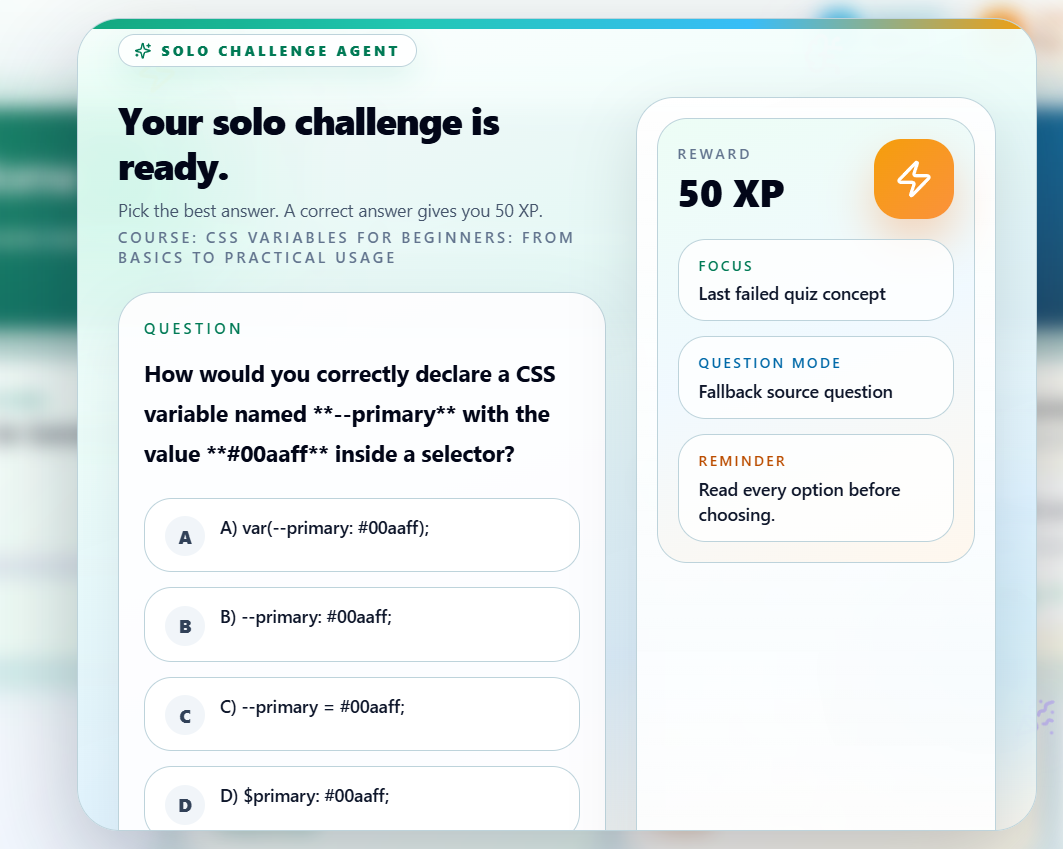
\includegraphics[width=0.75\textwidth]{figures/ch3_ai_solo_challenge_agent.png}%
        }{%
            \fbox{\parbox{0.85\textwidth}{\centering Figure à ajouter : challenge personnalisé généré pour l'apprenant et résultat après réponse.}}%
        }
        \caption{Challenge personnalisé généré par l'agent IA}
        \label{fig:ch3_ai_solo_challenge_agent}
    \end{figure}
\end{itemize}

En complément de ces cinq agents, un workflow de mémoire de cours est utilisé pour préparer les connaissances liées aux cours publiés. Il transforme les contenus pédagogiques, les leçons et les quiz en documents exploitables par la mémoire persistante. Ce mécanisme sert de support aux agents, notamment au coach IA, à l'agent de recommandation et à l'agent de challenge, car il leur fournit une base de connaissances structurée sur le contenu réel des cours.

\section{Déploiement et hébergement de la plateforme}

Le déploiement de la plateforme a été réalisé sur une machine virtuelle Linux mise à disposition par la société, afin d'assurer un environnement stable et proche des conditions de production. L'accès à la VM se fait via SSH, et l'ensemble des opérations d'administration (vérification système, déploiement et exécution) est effectué directement en ligne de commande.

La machine virtuelle dispose d'une configuration adaptée aux besoins du projet, avec environ 8 vCPU, 15 Go de mémoire RAM et un espace disque d'environ 23 Go (dont une partie libre pour le déploiement). Cette configuration est suffisante pour le fonctionnement de la plateforme dans un contexte de démonstration et de tests fonctionnels, tout en nécessitant une surveillance de l'espace disque lors de l'exécution des services conteneurisés.

Le déploiement repose sur une approche entièrement conteneurisée via Docker et Docker Compose, garantissant la cohérence entre l'environnement de développement et l'environnement d'hébergement. L'ensemble des services de la plateforme est orchestré sous forme de conteneurs, notamment : le frontend Next.js, les services backend, PostgreSQL avec extension pgvector, RabbitMQ, MinIO, ainsi que les services liés aux agents IA.

Le processus de déploiement comprend la récupération du code source depuis le dépôt Git, la configuration des variables d'environnement (JWT, base de données, URLs des services, clés d'accès et paramètres IA), puis le lancement de l'ensemble des services via Docker Compose. Cette approche permet de garantir une installation reproductible et centralisée de la plateforme.

Une fois les conteneurs démarrés, la plateforme est accessible via l'adresse IP de la VM, soit directement à travers le port exposé du frontend, soit via le point d'entrée configuré par le reverse proxy.

Enfin, l'architecture de déploiement reste évolutive et permet une migration future vers un environnement cloud plus robuste, tout en conservant les mêmes artefacts Docker et la même configuration, ce qui facilite la portabilité et la maintenance de la solution.

\section{Conclusion}

Ce chapitre a présenté la réalisation concrète des principaux modules de la plateforme, couvrant la gestion des identités, des formations, du mentorat, de la gamification et des agents d'intelligence artificielle. L'architecture décrite dans le chapitre précédent a été traduite en fonctionnalités opérationnelles, accessibles depuis les interfaces développées. Le déploiement a été préparé autour d'une approche conteneurisée, prête pour un hébergement sur VM. Les tests, l'évaluation des résultats et l'analyse des limites sont détaillés dans le chapitre suivant.
